\chapter{MNIST experiments}

\section{MNIST}

Jest to zbiór po kategoryzowanych odręcznie napisanych cyfr. Wszystkie obrazki są czarno-białe, rozmiaru 28x28 i wycentrowane. Zbiór składa się z 60000 danych treningowych i 10000 testowych. Zbiór ten często wykorzystywany jest w celach testowych. W sensie, że jeżeli model na nim nie zadziała, to z dużym prawdopodobieństwem nie zadziała również na bardziej skomplikowanych danych. Przykładowe obrazki \ref{fig:mnist}.

\begin{figure}[h!]
    \centering
    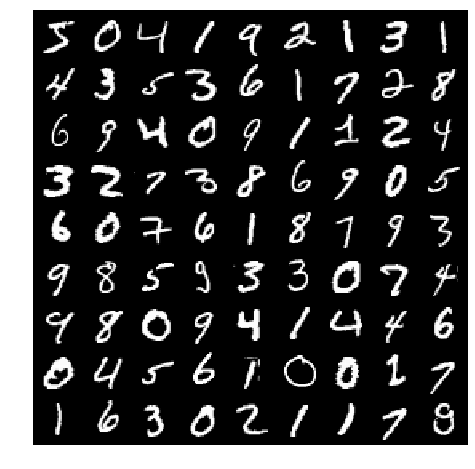
\includegraphics[width=0.4\textwidth]{images/mnist}
    \caption{Samples from MNIST dataset}
    \label{fig:mnist}
\end{figure}

\section{VAE}

Poniżej na rysunku \ref{fig:vae}


\begin{figure}[h!]
  \centering
  \begin{subfigure}[b]{0.57\linewidth}
    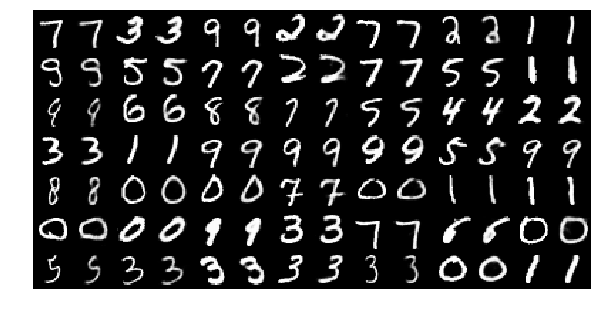
\includegraphics[width=\linewidth]{images/mnist_recon}
    \caption{Coffee.}
  \end{subfigure}
  \begin{subfigure}[b]{0.30\linewidth}
    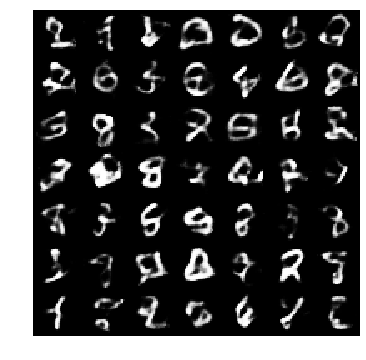
\includegraphics[width=\linewidth]{images/mnist_gen}
    \caption{More coffee.}
  \end{subfigure}
  \caption{The same cup of coffee. Two times.}
  \label{fig:vae}
\end{figure}

\begin{figure}
    \centering
    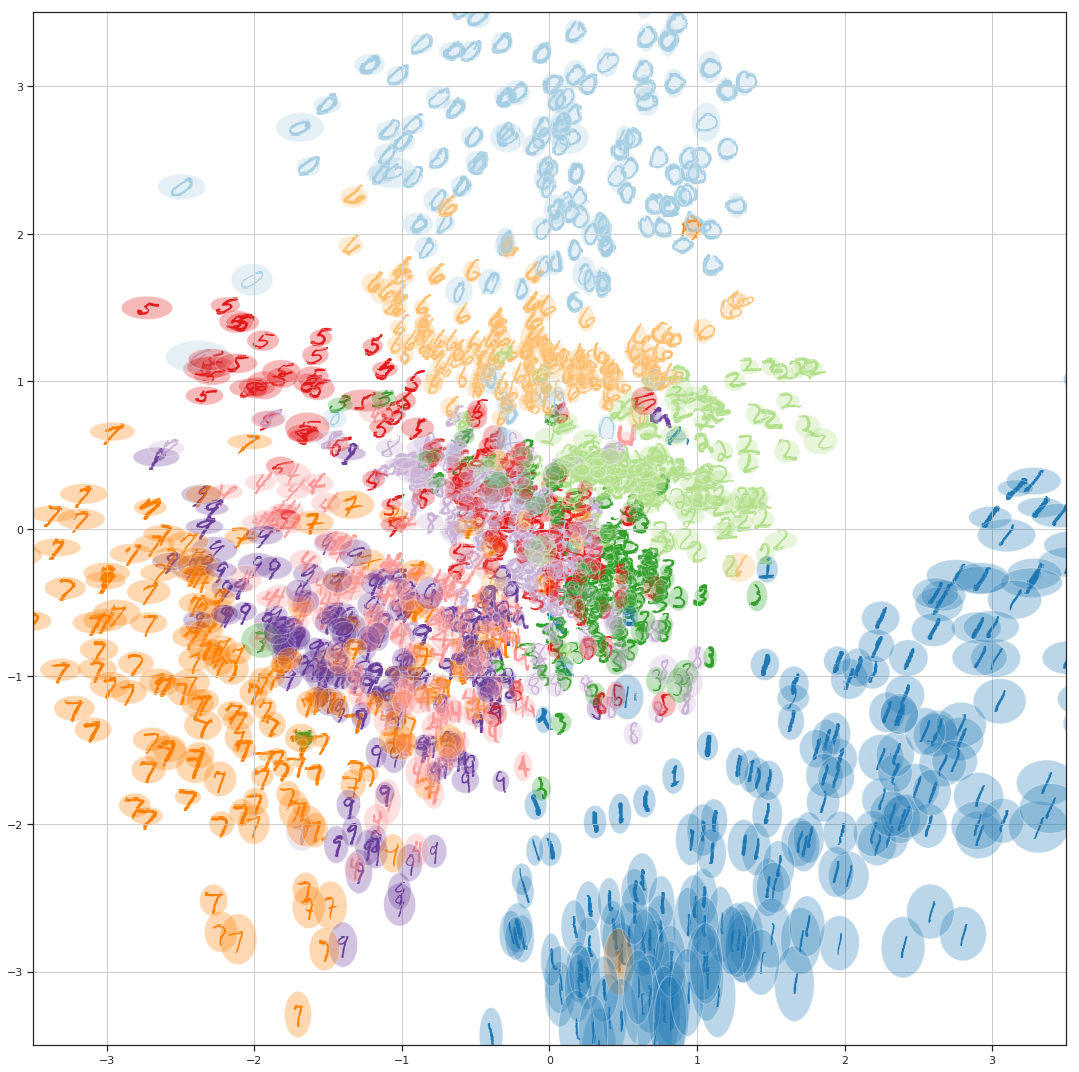
\includegraphics[width=0.7\textwidth]{images/mnist_2d}
    \caption{}
    \label{fig:mnist_2d}
\end{figure}

\begin{figure}
    \centering
    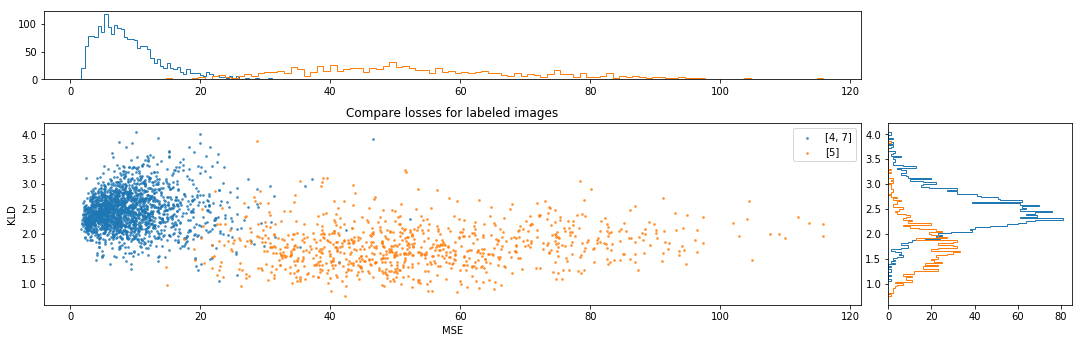
\includegraphics[width=1.0\textwidth]{images/mnist_compare}
    \caption{}
    \label{fig:mnist_compare}
\end{figure}

\begin{figure}
    \centering
    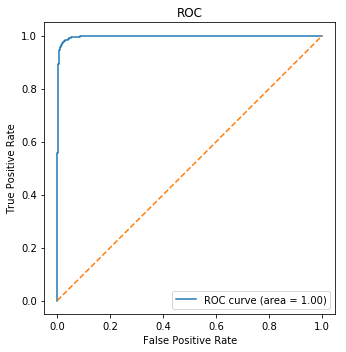
\includegraphics[width=0.6\textwidth]{images/mnist_roc}
    \caption{}
    \label{fig:mnist_roc}
\end{figure}

\section{Deep feature consistent variational auto-encoder}

Wyniki przy użyciu Deep feature consistent variational auto-encoder.

\begin{figure}
    \centering
    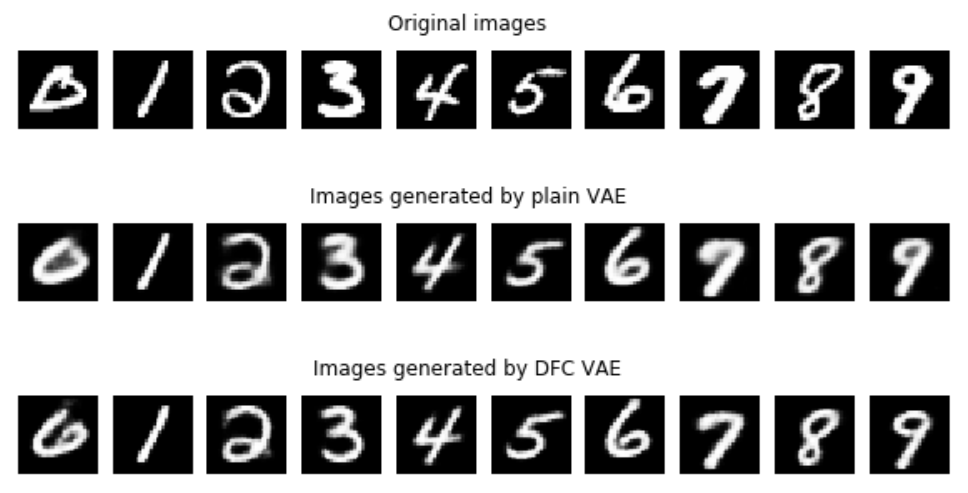
\includegraphics[width=1.0\textwidth]{images/vae_dfc_gen}
    \caption{}
    \label{fig:vae_dfc_gen}
\end{figure}

\begin{figure}
    \centering
    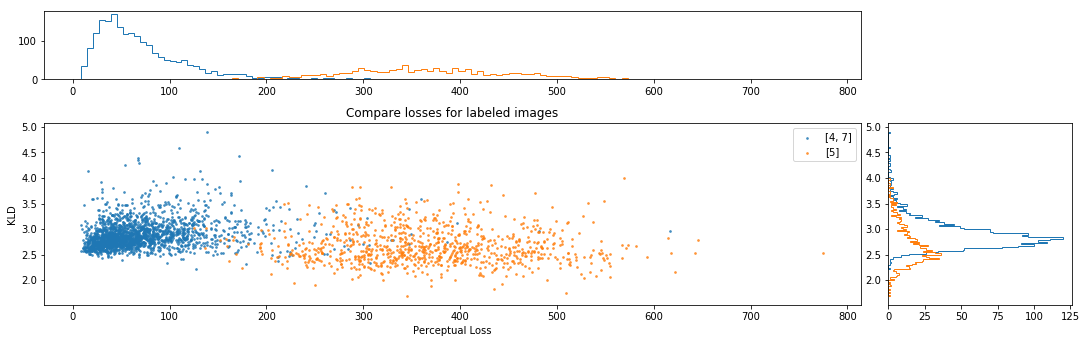
\includegraphics[width=1.0\textwidth]{images/dfc_mnist_compare}
    \caption{}
    \label{fig:dfc_mnist_compare}
\end{figure}
